\documentclass{beamer}

\usepackage[T2A]{fontenc}
\usepackage[russian]{babel}
\usepackage{paratype}
\usepackage{xcolor}
\usepackage{colortbl}
\usepackage{array}
\usepackage{tabularx}
\usepackage{booktabs}

\usepackage{mathtools}
\let\abs\relax
\DeclarePairedDelimiter\abs{\lvert}{\rvert}

\usetheme{Darmstadt}
\usecolortheme{seahorse}
\usefonttheme[onlymath]{serif}
\usepackage{marvosym}
\usepackage{tikz}
\usetikzlibrary{graphs}
\usetikzlibrary{shapes, arrows}
\tikzstyle{decision} = [
                diamond,
                draw,
                fill = green!20,
                text width = 6em,
                text badly centered,
                node distance = 2cm,
                inner sep = 0pt
        ]
\tikzstyle{block} = [
                rectangle,
                draw,
                fill = blue!20,
                text width = 7em,
                text centered,
                rounded corners,
                minimum height = 3em
        ]
\tikzstyle{block0} = [
                rectangle,
                draw,
                fill = yellow!10,
                text width = 13em,
                rounded corners,
                minimum width = 13em
        ]
\tikzstyle{line} = [
                draw,
                -latex'
        ]

%Более крупный шрифт для подзаголовков титульного листа
\setbeamerfont{institute}{size=\normalsize}

\newcommand{\col}{\textcolor[rgb]{0.2,0.,0.55}}

\AtBeginSection[]{
  \begin{frame}
  \vfill
  \centering
  \begin{beamercolorbox}[sep=8pt,center,shadow=true,rounded=true]{title}
    \LARGE\insertsectionhead\par%
  \end{beamercolorbox}
  \vfill
  \end{frame}
}

\AtBeginSubsection[]{
  \begin{frame}
  \vfill
  \centering
  \begin{beamercolorbox}[sep=8pt,center,shadow=true,rounded=true]{title}
    \usebeamerfont{title}\insertsubsectionhead\par%
  \end{beamercolorbox}
  \vfill
  \end{frame}
}

\begin{document}

\title{{Теория магического четырёхугольника}}
\author[%
	Назаров В.\ С. \and Фрайман М.\ И.
]{%
	\scriptsize
	Назаров В.\ С. \and Фрайман М.\ И.
}
\date{\footnotesize{Москва "--- 2019}}


	\begin{frame}
		\begin{center}
			\footnotesize{МГУ имени М. В. Ломоносова}\\
			\footnotesize{Механико-математический факультет}\\\vspace{10pt}
		\end{center}
		\titlepage
	\end{frame}

	\section{Общее описание}

	\begin{frame}{Что это такое}
	
		\textbf{Магический четырёхугольник} "--- это схема, иллюстрирующая основные цели экономической политики:
		\begin{itemize}
			\item Экономический рост (обычно "--- ВВП или ВНП);
			\item Полная занятость населения;
			\item Низкая инфляция;
			\item Платёжный баланс.
		\end{itemize}
		
	\end{frame}
	
	\begin{frame}{Собственно, сабж}
	
		\begin{center}
			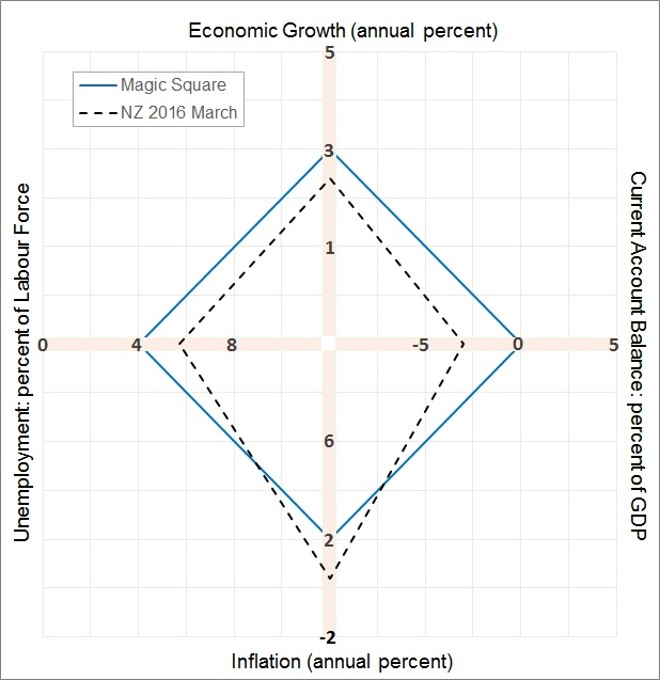
\includegraphics[height = .8\textheight]{ms.jpg}
		\end{center}
		
	\end{frame}
	
	\begin{frame}{Формула}
			\[
				\mathrm{MPI_{MS}} = \lambda_{\hat{y}}\cdot\hat{y} - 
									\lambda_\pi\cdot\abs*{\pi-\pi^T} +
									\lambda_{\mathrm{cab}}\cdot\abs*{{\mathrm{cab}}-{\mathrm{cab}}^T} -
									\lambda_u\cdot\abs*{u-u^T}
			\]
			
			\begin{itemize}
			\item $\lambda$ "--- веса, ассоциированные с параметрами;
			\item $\hat{y}$ "--- реальный ВВП на душу населения;
			\item $\pi$ "--- скорость инфляции;
			\item $\mathrm{cab}$ "--- баланс на счету;
			\item $u$ "--- уровень безработицы;
			\item индекс $T$ указывает на то, что параметр \textit{желаемый.}
			\end{itemize}
			
	\end{frame}

	\section{Почему ничего не работает (на~примере Израиля)}
	
	\begin{frame}{Попытка реализовать идеи Кейнса}
		Государственное обеспечение экономического роста осуществлялось по трём основным направлениям:
		\begin{itemize}
		\item государство прямо или косвенно являлось огромным источником спроса;
		\item с помощью субсидий оно создавало благоприятные условия для предпринимательства в целом;
		\item его структурная политика стимулировала импортозамещающее, а также ориентированное на экспорт производство и приток зарубежных инвестиций в динамично развивающиеся отрасли промышленности.
		\end{itemize}
	\end{frame}

	\begin{frame}{Итоги кейнсианских идей}
		Попытка реализовать идеи Кейнса привела к следующим проблемам.
		\begin{itemize}
			\item Малоэффективная промышленность;
			\item Снижение стимула к труду;
			\item Увеличение зависимости от государственной поддержки сопровождалось все новыми требованиями о её увеличении.
		\end{itemize}
	\end{frame}

	\begin{frame}{Переход к неоклассической политике}
		Был взят курс на резкое снижение экономической активности государства, поощрение конкуренции, всестороннюю либерализацию хозяйства.
		Предприняты шаги:
		\begin{itemize}
		\item Борьба с инфляцией;
		\item Сокращение бюджетного дефицита;
		\item Уменьшение субсидий.
		\end{itemize}
	\end{frame}
	
	\begin{frame}{Итоги неоклассических идей}
		Попытка реализовать неоклассические идеи привела к следующим проблемам.
		\begin{itemize}
			\item Платёжный баланс по текущим операциям был сведен с активным сальдо;
			%(надо посмотреть что это) ,
			\item Дефицит госбюджета сократился до~1\% от ВВП в среднем за период 1985--89~годов;
			\item Сокращение роста внутренней и внешней задолженности повысили доверие к израильскому шекелю.
		\end{itemize}
	\end{frame}

	\section{Выводы}

	\begin{frame}{Выводы}
		\begin{itemize}
			\item Вмешательство государства в экономику, способно эффективно решать только проблемы, стоящие в данный момент особенно остро;
			\item Долговременная помощь государства отдельным отраслям экономики снижает их эффективность и конкурентоспособность;
			\item При целенаправленном решении одних экономических проблем, возникают другие проблемы;
			\item Свободный рынок с ограниченным вмешательством государства обеспечивает наиболее эффективное экономическое развитие и условия «честной» конкуренции.
		\end{itemize}
	\end{frame}

\end{document}
